\documentclass[11pt]{article}
\usepackage[utf8]{inputenc} % Para caracteres en espa�ol
\usepackage{amsmath,amsthm,amsfonts,amssymb,amscd}
\usepackage{multirow,booktabs}
\usepackage[table]{xcolor}
\usepackage{fullpage}
\usepackage{lastpage}
\usepackage{enumitem}
\usepackage{multicol}
\usepackage{fancyhdr}
\usepackage{mathrsfs}
\usepackage{wrapfig}
\usepackage{setspace}
\usepackage{esvect}
\usepackage{calc}
\usepackage{multicol}
\usepackage{cancel}
\usepackage{graphicx}
\graphicspath{ {pictures/} }
\usepackage[retainorgcmds]{IEEEtrantools}
\usepackage[margin=3cm]{geometry}
\usepackage{amsmath}
\newlength{\tabcont}
\setlength{\parindent}{0.0in}
\setlength{\parskip}{0.05in}
\usepackage{empheq}
\usepackage{framed}
\usepackage{newtxmath}
\usepackage{euscript}
\DeclareMathAlphabet{\mathpzc}{T1}{pzc}{m}{it}
\usepackage[most]{tcolorbox}
\usepackage{xcolor}
\colorlet{shadecolor}{orange!15}
\parindent 0in
\parskip 12pt
\geometry{margin=1in, headsep=0.25in}
\theoremstyle{definition}
\newtheorem{defn}{Definition}
\newtheorem{reg}{Rule}
\newtheorem{exer}{Exercise}
\newtheorem{note}{Note}
\newcommand{\volume}{{\ooalign{\hfil$V$\hfil\cr\kern0.08em--\hfil\cr}}}
\newcommand{\parr}{\mathbin{\|}} % Parralel Symbol
\begin{document}
\setcounter{section}{0}
\setcounter{page}{2}
\setcounter{equation}{0}
%\definecolor{babyblue}{rgb}{0.54, 0.81, 0.94}
\definecolor{babyblueeyes}{rgb}{0.63, 0.79, 0.95}
\definecolor{babyblue}{rgb}{0.69, 0.88, 0.9}

 \pagestyle{fancy}
\fancyhf{}
\rhead{Section 6:  Ionization}
\rfoot{Page \thepage}
\thispagestyle{empty}

\begin{center}
{\LARGE \bf Section 6:  Ionization}\\
{\large AE435}\\
Spring 2018
\end{center}
\vspace{5mm}
\section{Equilibrium Ionization}
Here we derive the ionization fraction for an equilibrium gas.  This results in what is called the Saha Equation.
\vspace{10mm}
\tableofcontents
\newpage
\subsection{Detailed Balancing}
Assume \textbf{detailed balancing}, where every process is balanced by the reverse process:
 
 
Examples of the sort of reactions involved in detailed balancing:
 
  \begin{enumerate}
 \item  a
 \item a
 \end{enumerate}
 
 
The overall reaction can be described by an equilibrium constant
 
 
 
 
Can show from statistical mechanics that at equilibrium:
 \begin{shaded}
\textbf{State of Plasma}
 \begin{equation*}
 \begin{aligned}
 a
 \end{aligned}
 \end{equation*}
Where
 \begin{equation*}
 \begin{aligned}
 a & \text{ is the total population within the control volume} \\ 
 a & \text{ is the population within the CV at a given state, i} \\ 
 a & \text{ is the energy state ij} \\ 
  a & \text{ k is Boltzmann constant.} \\ 
 \end{aligned}
 \end{equation*}
 \end{shaded}

This determines the distribution among individual energy states at equilibrium. 



\newpage
\subsection{Partition Functions}
We can define a \textbf{total partition function} for a given species that is the product of a series of individual partial partition functions,
 
 
 
Where for each energy mode of a given species:
\begin{itemize}
\item Translational
\item Electronic
\item Rotational
\item Vibrational
\end{itemize}
We have a \textbf{partial partition function}
 
 
 
Jahn defines f  as the sum of accessible energy states, appropriately weighted by degeneracies and by the Boltzmann factors in the relative energies of those states.
 
Other ways of writing f include:
 
 
 
 
where       	is the ground-state energy. (Note: this is a more general form as it indicates that energy is relative                                                   
                                                                                                 )
 
 
 
 
includes the degeneracy      	, making it useful for electronic states.
 
The partition function is a link between classical thermo and the microscopic behavior of gases (statistical kinetic theory).  It is fairly easy to show that the total energy for N particles is:
 
 
 
For instance, the \textbf{translational partial partition function} is given on quantum mechanics basis, as (6.9) for atoms of mass MA:
 
 
 
 
Using (6.9), we can take
 
 
 
 
So that
 
 
 
The total translational energy is then:
 
 
 
which is the result we had before in section IV. A. 2. when we discussed Kinetic Theory and Internal Translational Energy.
 
 
Thus...
 
 \begin{shaded}
\textbf{electronic partial partition function}
 \begin{equation*}
 \begin{aligned}
 a
 \end{aligned}
 \end{equation*}
Where
 \begin{equation*}
 \begin{aligned}
 a & \text{ degeneracy for state j} \\ 
 a & \text{ represents the ground state} \\ 
 a & \text{ is the highest bound state} \\ 
 \end{aligned}
 \end{equation*}
 \end{shaded}
 
Note that this series converges rapidly, so we may need to only take a few terms at low to moderate temperature.  In hot plasmas, may need to take many terms for an accurate solution.
 
The \textbf{total atomic partition function} for species with negligible rotational and vibrational modes is:
 
 
Substituting in the partial partition functions,
 
 
 
Likewise, the \textbf{total ionic partition function}
 
 
becomes
 
 
We need to make sure that we have consistent assumptions about the energy reference state.  Doesn't matter what it is, but it has to be the same for all.

For atoms, we use the ground state,

For ions, we need to add the ionization energy to reference back to atomic ground, thus
 
 
where the following terms express an electronic energy level in the ion:

               	is referenced to the ionic ground state
	
               	is referenced to the atomic ground state
	
               	is the ionization energy (referenced to the atomic ground state)
 
The total electron partition function (for free electrons) is
 
 
where              	is the spin degeneracy (the only internal degree of freedom); substituting and using (6.9),
\newpage
\subsection{Saha Equation}
The equilibrium constant for ionization
 
 
 
can be expressed as the ratio of total partition functions,
 
 
Substituting in, using (6.20), (6.15), (6.17) and (6.18),
 
 
 
 
where
 
 
is the electronic partial partition function for ions, and
 
 
 
is  the electronic partial partition function for atoms.  This is the classic form of the Saha Equation from astrophysics (6.23).
 
An alternative form used often in gas dynamics started by defining the ionization fraction
 
 \begin{shaded}
\textbf{Ionization Fraction}
 \begin{equation*}
 \begin{aligned}
 a
 \end{aligned}
 \end{equation*}
Where
 \begin{equation*}
 \begin{aligned}
 a & \text{ is the ion density} \\ 
 a & \text{ is the neutral density} \\ 
 a & \text{ is the total density of heavy particles} \\ 
 \end{aligned}
 \end{equation*}
 \end{shaded}
 
If we assume quasineutrality
 
We can write
 
So the pressure from all 3 species (ions, atoms, electrons) is:
 
 
Substituting into the equilibrium constant equation (6.21)
 
 
where
 
\begin{shaded}
\textbf{SAHA Equation}
 \begin{equation*}
 \begin{aligned}
 a
 \end{aligned}
 \end{equation*}
 \end{shaded}
 
Can plot for argon:

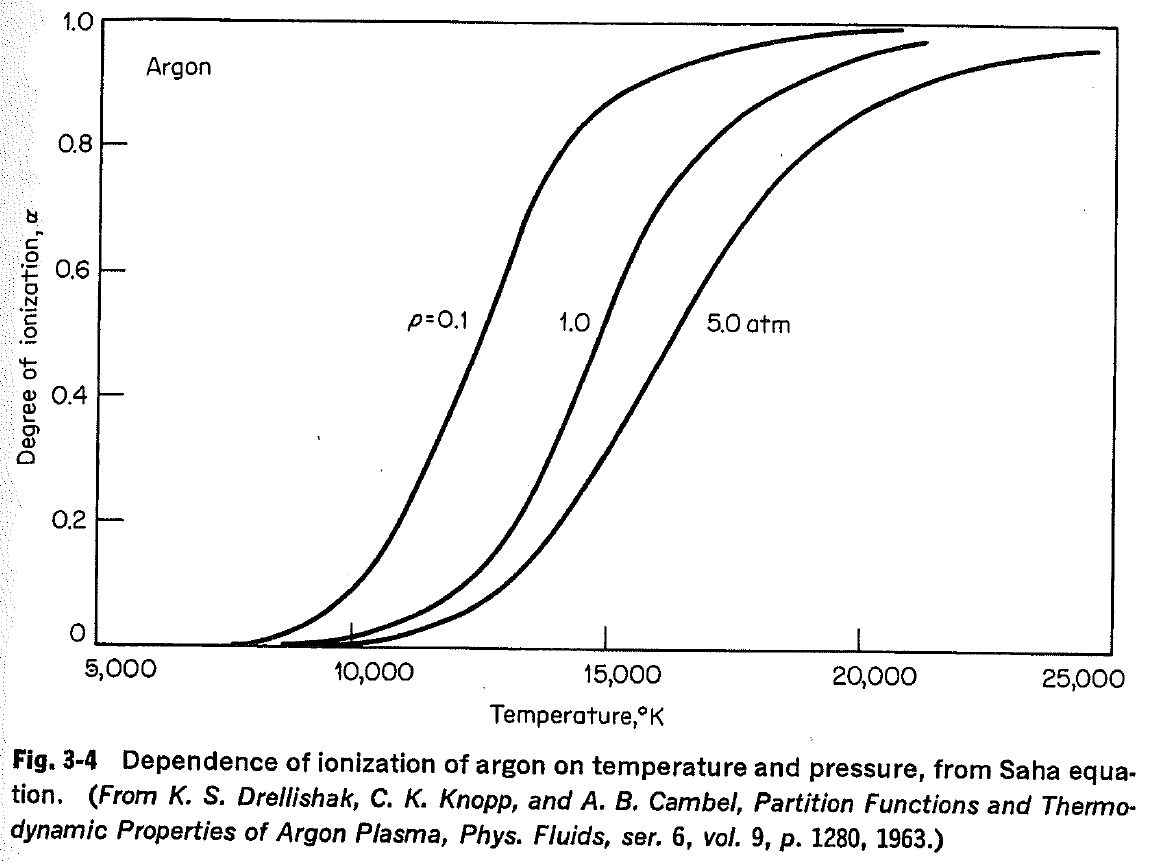
\includegraphics[scale=0.5]{1.png}
 
Note that collisional recombination drives the ionization fraction down at higher pressures.
 
Jahn gives a more complex analysis, required for multiple species and internal degrees of freedom.  Main points:
\begin{itemize}
\item Vibration and rotation require their associated partition functions
\item Additional reactions (dissociation, etc) can be handled the same way
\item Multiple ionization (high temp, low density) adds partition function and number of reactions
\end{itemize}
\newpage
\subsection{Conditions for Equilibrium}
Above analysis assumes \textbf{complete thermodynamic equilibrium (CTE)}:
\begin{enumerate}
\item Single temperature
\item Homogeneous plasma
\item Radiation field follows blackbody distribution

 
 
 
 
where     	is the radiation intensity (energy per unit time per u nit area per unit solid angle) and    	is the vacuum speed of light.  Note that this requires an optically thick plasma, where all radiation is absorbed and re-radiated multiple times (as in Sun's interior).
 
 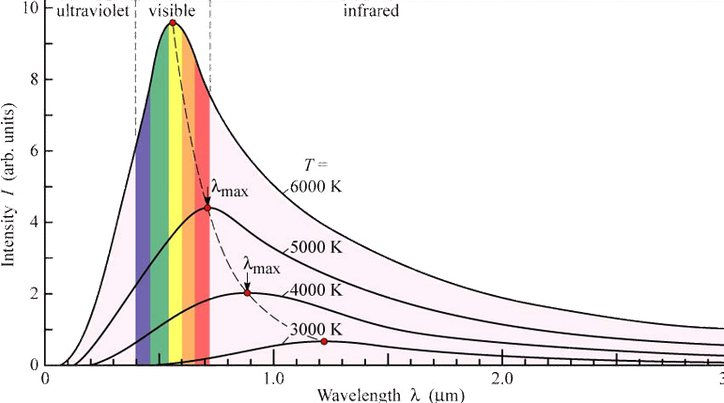
\includegraphics[scale=0.6r]{2.png}
 
\item Maxwellian-Boltzmann energy distribution.  Which follows from the Maxwellian velocity (speed) distribution (4.30).
 \end{enumerate}
 
 
 
For Te = 2eV electrons

  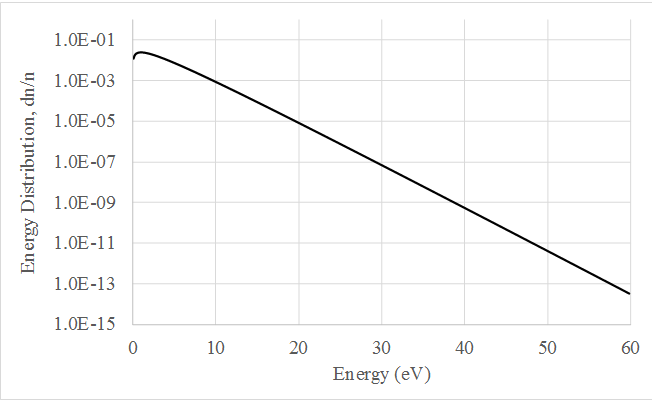
\includegraphics{3.png}
 
Note that the slope varies inversely with the temperature, we use this in several diagnostics (Langmuir probes, atomic Boltzmann method in optical emission spectroscopy) to measure plasma temperature.
In terms of speed,
 
 
And, again, the mean speed for a Maxwellian is:
 
 
 
In CTE,
\begin{itemize}
\item All ionization follows the Saha equation
\item All excitation follows the Boltzmann equation
\end{itemize}
 
 
\subsubsection{Deviations from Equilibrium}
\begin{enumerate}
    \item Local thermodynamic equilibrium (LTE), where plasma is
    \begin{itemize}
        \item Sufficiently dense that collisions are dominant populating mechanism
        \item Optically thin, so radiation field is nonequilibrium, can't use Planck's law
        \item Radiative processes do not follow detailed balancing, assume we can ignore radiation processes, plasma is collision determined.
    \end{itemize}
    In LTE, radiative emission dominates over absorption and photoionization, depleting the number of free electrons and excited states.  LTE is frequently encountered in lab plasmas.
    \item Partial local thermodynamic equilibrium (PLTE), where plasma is lower density:
    \begin{itemize}
    	\item Collisions are in detailed balance for upper energy levels
    	\item Collisions are not in detailed balance for transitions to the ground state
    	\item Often Ti < Te
    \end{itemize}
    As a result, upper energy levels follow Boltzmann distribution, but the ground state is overpopulated.  Again, depletes the free electron density.
    \item Non-equilibrium Plasma
    \begin{itemize}
    \item Multi-thermal "equilibrium"
    
    where we have a two-temperature plasma.  Typically:
     
     
    The reason for this is electron-impact collisions are an efficient method to transfer energy to gas, but a poor method of transferring momentum.  So atoms get energy from electron to become ionized (takes ionization energy), but they don't get momentum, so their translational energy (temperature) doesn't change.
     
    Fluorescent lights work by electron-impact excitation of mercury atoms.  (The dominant lines are in the UV, but coatings in the tube walls downconvert to visible light).  Temperatures:
    \begin{itemize}
        \item Gas, 300 K ~ 1/40 eV
        \item Electrons, 3.5 eV ~ 35,000 K
    \end{itemize}
    Collisional processes are often dominated by electrons, so we can get LTE or PLTE where the relevant temperature is Te.
     
    \item Corona "equilibrium"
    
    Note really a true equilibrium, as there is no detailed balancing.  Characteristics:
    \begin{itemize}
        \item Very low density plasmas
        \item Radiative decay rates >> collisional decay rates
        \item Optically thin
        \item Radiative excitation and ionization << collisional excitation and ionization
    \end{itemize}
    In this case we can balance
    
    Energy in by collisions = energy out by radiation
    
    For charge states Z and Z+1, the ionization balance is then:
     
     
    where
    
             	is the radiative recombination rate [s-1]
    	
             	is the electron-impact ionization rate [s-1]
    	
    Rearranging we get a simple relation for the corona model,
    
     
     
     
    which you'll note is independent of ne.
\end{enumerate}
\end{document}